\section{Application}
	\subsection{Presentation}
	
	Here we will present the look of our application, and describe its functionnalities. In the \textsc{Figure} \ref{fig:general} we can see the welcoming screen of the guide.
	It has :
	\begin{enumerate}
		\item A title;
		\item A data entering zone;
		\item A welcoming map.
	\end{enumerate}
		\begin{figure}[h!]
			\centering
			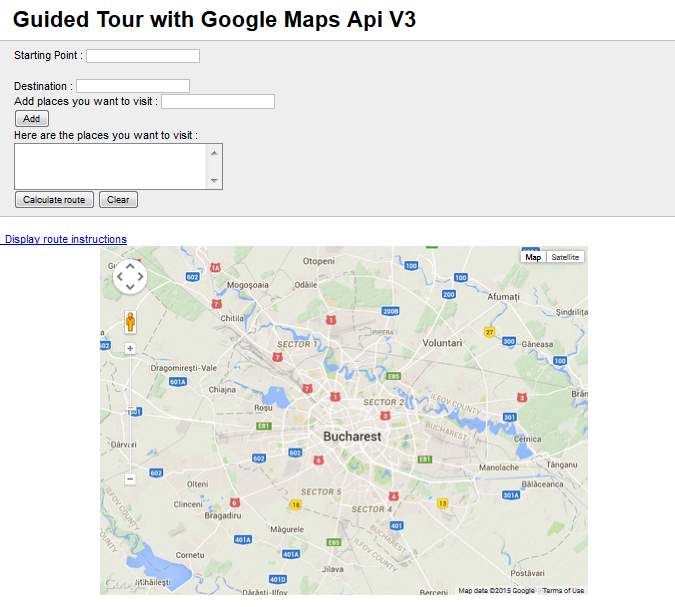
\includegraphics[scale=0.7]{input/general_look.png}
			\caption{\label{fig:general}General look of the application.}
		\end{figure}
		
		If HTML5 geolocation is not enabled by default on your browser, or if you ask for each time a website wants to access if, you may see the pop-up in \textsc{Figure} \ref{fig:geoloc}, asking you to enable this feature.
		\begin{figure}[h!]
			\centering
			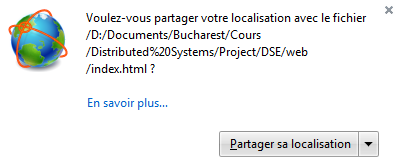
\includegraphics{input/geoloc.png}
			\caption{\label{fig:geoloc}Pop-up asking for your location.}
		\end{figure}
		
		If you decide to enable it, the welcoming map will display your position, as shown in the \textsc{Figure} \ref{fig:geoloc_map}.
		\begin{figure}[h!]
			\centering
			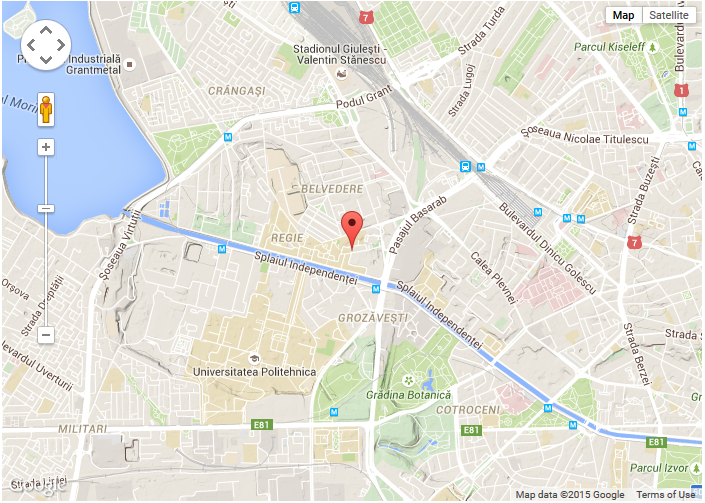
\includegraphics[scale=0.7]{input/geoloc_map.png}
			\caption{\label{fig:geoloc_map}Map showing your position.}
		\end{figure}
		
		Once the welcoming page reached, you can start using the application. It is very simple, you should follow these steps :
		\begin{enumerate}
			\item Enter a starting point;
			\item Adding an arrival point;
			\item Add the intermediate points you want to reach by entering one by one the points, and clicking the "Add" button.
			\item Click the "Calculate button"
		\end{enumerate}
		
		\begin{figure}[h!]
			\centering
			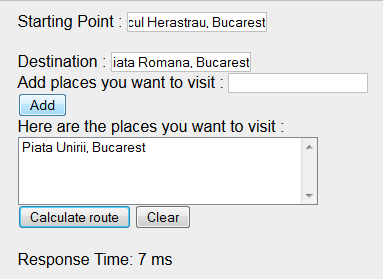
\includegraphics[scale=0.7]{input/make_route.png}
			\caption{\label{fig:route}How to use the application.}
		\end{figure}
		
		The route you should follow is displayed on the map
		
		\begin{figure}[h!]
			\centering
			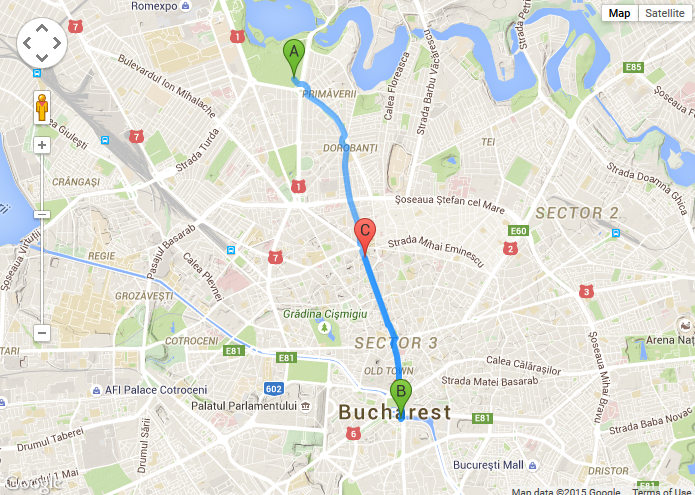
\includegraphics[scale=0.7]{input/map_result.png}
			\caption{\label{fig:general}Map displaying your optimized way through the points wanted.}
		\end{figure}
		
		\begin{figure}[h!]
			\centering
			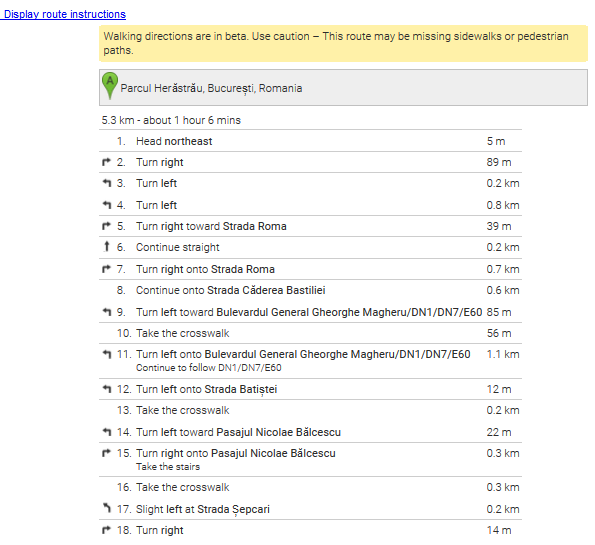
\includegraphics[scale=0.9]{input/instructions.png}
			\caption{\label{fig:general}You can display the specific directions.}
		\end{figure}
		
		\newpage\subsection{Technologies}
			\begin{itemize}
				\item NetBeans
				\item Google Maps API
				\item JS
			\end{itemize}